\documentclass{article}

\usepackage[utf8]{inputenc}
\usepackage{enumerate}
\usepackage{graphicx}

\title{\textbf{Mecánica computacional - Trabajo Práctico 2}}
\author{FILARDI, Esteban; VICTORIO, Franco}
\date{}

\begin{document}

\maketitle

\begin{enumerate}[1)]
    \item{ % 1)
        En los dos casos se usa:

        \[ \psi = x + 1 \]
        \[ N_m(x) = \sin(m \pi x) \]

        El error utilizado es:

        \[ \mbox{error} = \frac{\left|\left| x_{aprox} - x_{exacta}\right|\right|_2}{\left|\left| x_{exacta} \right|\right|_2} \]

        evaluando en $1000$ puntos equiespaciados en $[0, 1]$.

        \vspace{0.5cm}

        \textbf{Colocación puntual}: usando $M$ puntos equiespaciados
        y en el interior del dominio (para $M=2$ los puntos 
        $\frac{1}{3}$ y $\frac{2}{3}$, por ejemplo), se obtienen los
        siguientes resultados:

        \begin{tabular}{|c|c|c|}
        \hline
        \textbf{M} & \textbf{Error} & \textbf{Proporción mejora} \\
        \hline
        1 & 5.1067e-01 & \\
        \hline
        2 & 1.6125e-01 & 3.1670 \\
        \hline
        4 & 4.1164e-02 & 3.9173 \\
        \hline
        8 & 9.1047e-03 & 4.5212 \\
        \hline
        16 & 1.8320e-03 & 4.9697 \\
        \hline
        32 & 3.4760e-04 & 5.2706 \\
        \hline
        \end{tabular}

        \vspace{0.5cm}

        \textbf{Galerkin}: con el método de Galerkin se obtienen
        los siguientes resultados:

        \begin{tabular}{|c|c|c|}
        \hline
        \textbf{M} & \textbf{Error} & \textbf{Proporción mejora} \\
        \hline
        1 & 9.4531e-03 & \\
        \hline
        2 & 2.8715e-03 & 3.2921 \\
        \hline
        4 & 6.8859e-04 & 4.1701 \\
        \hline
        8 & 1.4254e-04 & 4.8309 \\
        \hline
        16 & 2.7272e-05 & 5.2267 \\
        \hline
        32 & 5.0146e-06 & 5.4384 \\
        \hline
        \end{tabular}

        \vspace{0.5cm}

        A continuación se muestran las gráficas para ambos métodos en el
        caso $M=2$:

        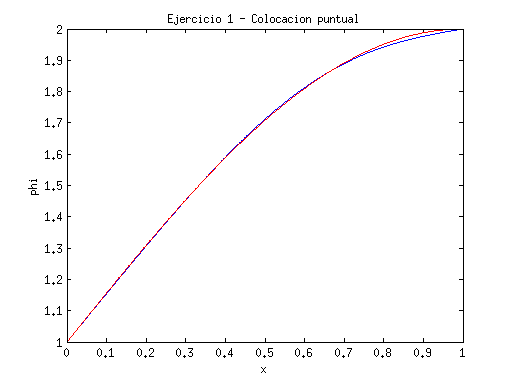
\includegraphics[width=\textwidth]{ej1_cp.png}

        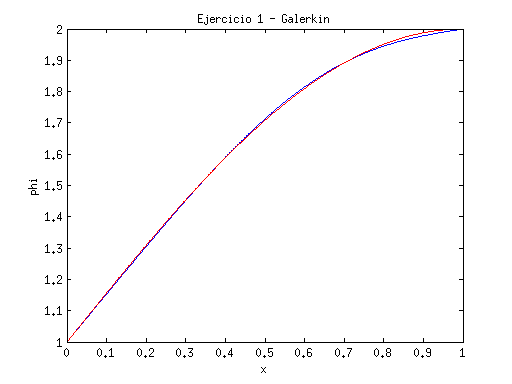
\includegraphics[width=\textwidth]{ej1_galerkin.png}
    }
    \item{ % 2)
        La solución exacta al problema dado es:

        \[ \phi(x) = \frac{1 + \sin(1) - \cos(1)}{\cos(1) + \sin(1)} \sin(x) + \cos(x) - 1 \]

        Usando el método de los resiudos ponderados puede obtenerse una solución aproximada
        de la forma $\psi + \sum_{m=1}^M a_m N_m$. Dado que hay una condición Dirichlet
        y una Neumann, la primera se satisface haciendo $\psi = 0$ y $N_m|_{x=0} = 0$.
        La condición Neumann se incluye en el residuo:

        \[ R_\Omega = \frac{\mbox{d}^2\hat{\phi}}{\mbox{d}x^2} +
                      \hat{\phi} + 1 \]

        \[ R_\Gamma = \hat{\phi} + \frac{\mbox{d}^2\hat{\phi}}{\mbox{d}x^2} \]

        Usando Galerkin, se llega a:

        \[ K_{lm} = \int_0^1{\frac{\mbox{d}N_l}{\mbox{d}x} \frac{\mbox{d}N_m}{\mbox{d}x} \mbox{d}x} + 
                    \int_0^1{N_l N_m \mbox{d}x}
                    \int_0^1{\mbox{d}x} - [N_l N_m]_{x=1} \]

        \[ f_l = -\int_0^1{N_l \mbox{d}x} \]

        Utilizando $N_m = x^m$ para $m = 1, 2, \ldots$ como funciones de forma se obtienen las 
        siguientes gráficas:

        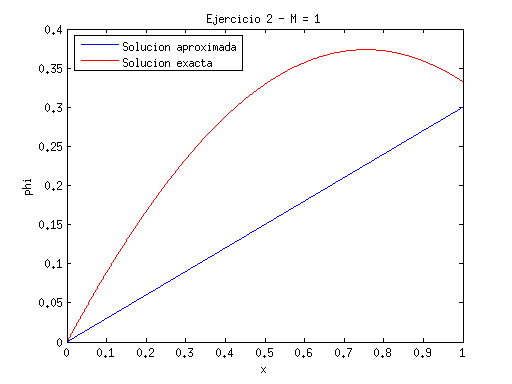
\includegraphics[width=\textwidth]{ej2_M_1.png}

        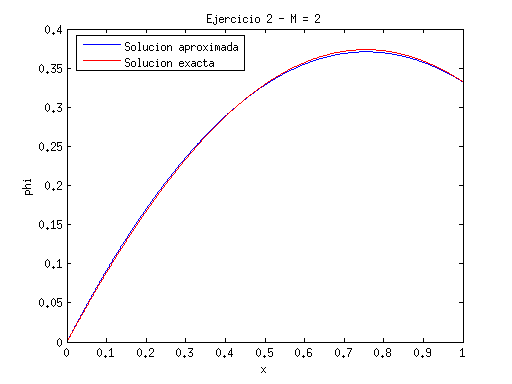
\includegraphics[width=\textwidth]{ej2_M_2.png}
    }
\end{enumerate}
\end{document}
